%%%%%%%%%%%%%%%%%%%%%%%%%%%%%%%%%%%% Chapter Template

\chapter{Optimization} 	% Main chapter title
\label{Chapter2} 		% For referencing the chapter elsewhere, usage \ref{Chapter1}

%%%%%%%%%%%%%%%%%%%%%%%%%%%%%%%%%%%%

Following the design of the R1 V5 Satori 3 and discussions with the Ozone paragliding design team, my attention turned to enhancing the performance of the kite. To achieve this, I collaborated with Fred Pieri, a paraglider designer, to develop an optimization algorithm. This algorithm, written in Python, makes use of the Aerosandbox library.

%%%%%%%%%%%%%%%%%%%%%%%%%%%%%%%%%%%%%%%%%%%%%%%%%%%%%%%%%%%%%%%%%%%%%%%%%%%%%%%%
%%%%%%%%%%%%%%%%%%%%%%%%%%%%%%%%%%%% SECTION 1 %%%%%%%%%%%%%%%%%%%%%%%%%%%%%%%%%
%%%%%%%%%%%%%%%%%%%%%%%%%%%%%%%%%%%%%%%%%%%%%%%%%%%%%%%%%%%%%%%%%%%%%%%%%%%%%%%%

\section{Aerosandbox}
\label{sec:Ch2.1}

AeroSandbox\cite{aerosandbox} is a Python package that helps designing and optimizing aircrafts and other engineered systems. It is developed by Peter Sharpe, a graduate student studying aircraft design, multidisciplinary design optimization (MDO) and applied aerodynamics in MIT's Department of Aeronautics and Astronautics.

At its heart, AeroSandbox is an optimization suite that combines the ease-of-use of familiar NumPy syntax with the power of modern automatic differentiation.

This automatic differentiation dramatically improves optimization performance on large problems: design problems with tens of thousands of decision variables solve in seconds on a laptop. AeroSandbox also comes with dozens of end-to-end-differentiable aerospace physics models, allowing users to simultaneously optimize an aircraft's aerodynamics, structures, propulsion, mission trajectory, stability, and more.

%%%%%%%%%%%%%%%%%%%%%%%%%%%%%%%%%%%% SUBSECTION 1
\subsection{The 2D aerodynamics}
\label{sub:Ch2.1.1}

The 2D study uses \textbf{"NeuralFoil"}. It is a tool for rapid aerodynamics analysis of airfoils, similar to XFoil. Under the hood, NeuralFoil consists of physics-informed neural networks trained on tens of millions of XFoil runs.

NeuralFoil is 10 times faster than XFoil for a single analysis, and 1000 times faster for multipoint analysis, all with minimal loss in accuracy compared to XFoil. Due to the wide variety of training data and the embedding of several physics-based invariants, this accuracy is seen even on out-of-sample airfoils (i.e., airfoils it wasn't trained on). \cite{neuralfoil}

It uses the 2D Panel Method. It is a computational technique used in aerodynamics to analyze the flow of fluids around two-dimensional objects.
Here is a basic overview of how the 2D Panel Method works:
\begin{itemize}
    \item Discretization: The surface of the object is divided into a series of panels, which are typically flat or slightly curved. These panels represent small segments of the object's surface.
    \item Vortex Elements: Each panel is then modeled as a vortex element that produces a velocity field at its position. These elements create a mathematical representation of how the fluid interacts with the object's surface.
    \item Superposition Principle: The key idea behind the Panel Method is that the total velocity at any point in the flow field is the sum of the velocities induced by all the panels. This is based on the principle of superposition, which allows you to add up the effects of individual panels to obtain the overall flow field.
    \item Kutta Condition: To ensure the accuracy of the method, a condition called the Kutta condition is applied at the trailing edge of the airfoil. This condition ensures that the flow separates smoothly from the trailing edge, which is physically realistic. (i.e. the flow circulation is conserved).
    \item Computational Solution: The method involves solving a system of linear equations to satisfy the boundary conditions at the surface of the object (normal velocity is equal to zero) and the Kutta condition at the trailing edge. Once this system is solved, it provides the velocity distribution around the object and can be used to calculate various aerodynamic parameters such as lift, drag, and pressure distribution.
\end{itemize}

The 2D Panel Method is especially useful for preliminary design and analysis. While it simplifies certain aspects of fluid dynamics, it can provide valuable insights and accurate results for many practical engineering applications.

%%%%%%%%%%%%%%%%%%%%%%%%%%%%%%%%%%%% SUBSECTION 2
\subsection{The 3D aerodynamics}
\label{sub:Ch2.1.2}

The 3D study uses the \textbf{"Vortex Lattice Mathod (VLM)"}. It is a simplified mathematical approach that provides an approximate solution to the flow field around these objects. VLM is particularly useful for low-speed and subsonic aerodynamic analyses. Here is a basic overview of how the Vortex Lattice Method works:
\begin{itemize}
    \item Discretization: The surface of the aerodynamic object is divided into a set of smaller, interconnected panels or segments. These panels are often assumed to be flat and have a constant strength vortex associated with them.
    \item Vortex Representation: Each panel generates a vortex, and these vortices collectively form a lattice that represents the overall geometry of the object. The strength and location of these vortices are determined based on the local flow conditions and geometry.
    \item Induced Velocities: The induced velocity at any point in the flow field, caused by all the vortices in the lattice, is calculated using mathematical equations. This induced velocity represents how the vortices affect the flow at a particular location.
    \item Boundary Conditions: The VLM considers boundary conditions, such as the no-slip condition at the object's surface and the freestream velocity far from the object.
    \item Solution for Aerodynamic Forces: Using the induced velocities and boundary conditions, the method calculates aerodynamic forces and moments on the object, such as lift, drag, and pitch moment.
\end{itemize}

It's important to note that the Vortex Lattice Method is a simplified approach and comes with certain limitations. For instance, it assumes steady, incompressible, and inviscid flow, neglecting turbulence effects and compressibility. As such, it is most suitable for preliminary design and analysis where a quick assessment of an object's aerodynamic characteristics is needed. Despite its simplifications, the Vortex Lattice Method has been widely used in the early stages of aircraft design and in the analysis of various aerodynamic configurations due to its efficiency and ability to provide valuable insights into the behavior of aerodynamic systems.

Note that Aerosandbox also offers to use the \textbf{"Lifting Line Theory"} (LLT). It is a more advanced analytical method than the VLM used to calculate the lift distribution along the span of a finite wing. It considers the variation in lift across the wing, taking into account the effects of downwash and induced drag. The LLT relies on the concept of vortex filaments to model the lift distribution and uses integral equations to determine the lift characteristics of the wing.

%%%%%%%%%%%%%%%%%%%%%%%%%%%%%%%%%%%% SUBSECTION 3
\subsection{The geometry}
\label{sub:Ch2.1.3}

The three main geometry objects used in this study are the "Airplane", the "Airfoil" and the "Kulfan Airfoil".

\begin{itemize}
    \item The Airplane : it encapsulates the entire aircraft, comprising a collection of "Wing" objects, which constitute integral parts of the aircraft and are described by a list of sections, each featuring position, airfoil, twist angle, and chord parameters. Additionally, there is a list of "Fuselage" objects, which are also integral components of the aircraft and are associated with reference values.
    \item The Airfoil : It can be defined using either a set of coordinates or a NACA airfoil.
    \item The Kulfan Airfoil : the class shape transformation (CST) (Kulfan, 2008) is a popular airfoil parameterization \cite{Kulfan}.It generates a shape using Bernstein polynomials to scale a class function, which is most often a base airfoil shape. They are built with "lower weights" (8 points), "upper weights" (8 points), "leading edge weight" (1 point) and a trailing edge thickness. This class has recently been added (August 2023) to Aerosandbox in order to allow 2D airfoil optimization.   
\end{itemize}

%%%%%%%%%%%%%%%%%%%%%%%%%%%%%%%%%%%% SUBSECTION 4
\subsection{The optimization}
\label{sub:Ch2.1.4}

The Aerosandbox optimization part uses \textbf{"CasADi"}, an open-source software tool for numerical optimization in general and optimal control (i.e. optimization involving differential equations) in particular \cite{Andersson2018}. It solves the optimization problems using CasADi with IPOPT backend. 

\textbf{"Interior Point OPTimizer, pronounced I-P-Opt"} (IPOPT) is a software library for large scale nonlinear optimization of continuous systems \cite{ipopt}. IPOPT implements a \textbf{primal-dual interior point method}, and uses line searches based on Filter methods (Fletcher and Leyffer).

Primal-dual interior point method has the advantages of :
\begin{itemize}
    \item efficiency for large-scale problems (can handle problems with a large number of variables and constraints)
    \item global convergence (can find solutions that are globally optimal or nearly optimal) 
    \item handling inequality constraints
    \item well-suited for linear and convex problems
    \item predictable convergence behavior
\end{itemize}

but also has the disadvantages of :
\begin{itemize}
    \item lack of flexibility (primarily designed for convex optimization problems)
    \item sensitivity to initial conditions
    \item computational cost
    \item limited support for non-smooth functions (functions that have continuous derivatives of all orders)
\end{itemize}

Consequently, although certain drawbacks, such as computational cost and sensitivity to initial conditions, were encountered in its utilization, the primal-dual interior point method continued to prove highly suitable for this specific application.


% Here is a basic overview of how the \textbf{primal-dual interior point method} works :

% Starting from a nonlinear optimization problem with inequality constraints:
% \begin{equation}
%     \left\{
%     \begin{array}{ll}
%         minimize & f(x) \\
%         subject\: to & x \in \mathbf{R}^{N} \\
%         & c_{i}(x) \geq 0, for\: i=1,...,m \\
%         where & f:\mathbf{R}^{N} \rightarrow \mathbf{R}, c_{i}:\mathbf{R}^{N} \rightarrow \mathbf{R}
%     \end{array}
% \right.
% \label{eq:non linear optimization problem}
% \end{equation}

% The primal-dual interior point method solves an inequality-constrained optimization problem by converting it into an unconstrained objective function whose minimum we hope to find efficiently. Specifically, the logarithmic barrier function associated with \ref{eq:non linear optimization problem} is :
% \begin{equation}
%     B(x,\mu) = f(x) - \mu \sum_{i=1}^{m} log(c_{i}(x))
% \label{eq:logarithmic barrier function}
% \end{equation}

% Then, using the gradient of the barrier function and, in addition to the original ("primal") variable x, introducing a Lagrange multiplier-inspired dual variable $\lambda \in \mathbf{R}^{m}$ :
% \begin{equation}
%     c_{i}(x) \lambda _{i} = \mu, \forall i =1,...,m
%     \label{eq:Lagrange multiplier-inspired dual variable}
% \end{equation}
% we try to find the $(x_{\mu}, \lambda_{\mu})$ for which the gradient of the barrier function is zero.

% We get an equation for the gradient : 
% \begin{equation}
%     \nabla B(x_{\mu}), \lambda_{\mu} = \nabla f(x_{\mu}) - \mu \sum_{i=1}^{m} \frac{1}{c_{i}(x_{\mu})} \nabla c_{i}(x_{\mu}) = \nabla f(x_{\mu}) - J(x_{\mu})^{T} \lambda_{\mu} = 0
%     \label{eq:equation for the gradient}
% \end{equation}

% where the matrix J is the Jacobian of the constraints c(x).

% The intuition behind \ref{eq:equation for the gradient} is that the gradient of f(x) should lie in the subspace spanned by the constraints' gradients. The "perturbed complementarity" \ref{eq:Lagrange multiplier-inspired dual variable} with small $\mu$  can be understood as the condition that the solution should either lie near the boundary $c_{i}(x) = 0$, or that the projection of the gradient $\nabla f$ on the constraint component $c_{i}(x)$ normal should be almost zero.

% Applying Newton's method to \ref{eq:Lagrange multiplier-inspired dual variable} and \ref{eq:equation for the gradient}, we get the equation where appear H, the Hessian matrix of $B(x,\mu)$ and diag(), diagonal matrices : 
% \begin{equation}
%     \begin{pmatrix}
%         H(x,\lambda) & -J(x)^{T}\\
%         diag(\lambda)J(x) & diag(c(x))
%     \end{pmatrix}
%     \begin{pmatrix}
%         p_{x}\\
%         p_{\lambda}
%     \end{pmatrix} = 
%     \begin{pmatrix}
%         -\nabla f(x) + J(x)^{T} \lambda\\
%         \mu - diag(c(x))\lambda
%     \end{pmatrix}
%     \label{eq:equation for the search direction for iteratively updating }
% \end{equation}  

% Here, $(p_{x},p_{\lambda})$ is the search direction for iteratively updating $(x, \lambda)$.

% Because of \ref{eq:non linear optimization problem} and \ref{eq:Lagrange multiplier-inspired dual variable} the condition $\lambda \geq 0$ should be enforced at each step. This can be done by choosing appropriate $\alpha$ : 
% $(x, \lambda) \rightarrow (x+\alpha p_{x}, \lambda + \alpha p_{\lambda})$

%%%%%%%%%%%%%%%%%%%%%%%%%%%%%%%%%%%%%%%%%%%%%%%%%%%%%%%%%%%%%%%%%%%%%%%%%%%%%%%%
%%%%%%%%%%%%%%%%%%%%%%%%%%%%%%%%%%%% SECTION 2 %%%%%%%%%%%%%%%%%%%%%%%%%%%%%%%%%
%%%%%%%%%%%%%%%%%%%%%%%%%%%%%%%%%%%%%%%%%%%%%%%%%%%%%%%%%%%%%%%%%%%%%%%%%%%%%%%%

\section{2D optimization}
\label{sec:Ch2.2}

The 2D optimization algorithm was developed with the objective of improving the airfoil profile beyond that of the R1 V5 Satori 3, starting with the same base profile and introducing variations to the four parameters on the upper surface. The decision was made to retain the lower surface of the R1 V5 Satori 3 since it exhibited a "realistic" shape that yielded favorable results. The optimization program in Python incorporated the following conditions : 
\begin{itemize}
    \item The Cl must stay superior to the initial airfoil ones at few angles of attack ( 0°, 2.5°, 5°, 7.5°, 10°, 12.5°, 15°)
    \item The trailing edge angle must be superior or equal to the initial airfoil one
    \item The local thickness must stay positive
    \item The $\frac{d^{2}}{d^{2}_{x}}$ of the local thickness must stay negative
    \item The $\frac{d^{2}}{d^{2}_{x}}$ of the local camber must stay negative
    \item The $\frac{d}{d_{x}}$ of the upper coordinates must stay negative after the upper apex
    \item The $\frac{d}{d_{x}}$ of the lower coordinates must stay positive after the lower apex
    \item the maximum thickness must be superior or equal to 19\% of the chord
\end{itemize}

The following result was reached after 4 secondes :
\begin{figure}[H]
    \centering
    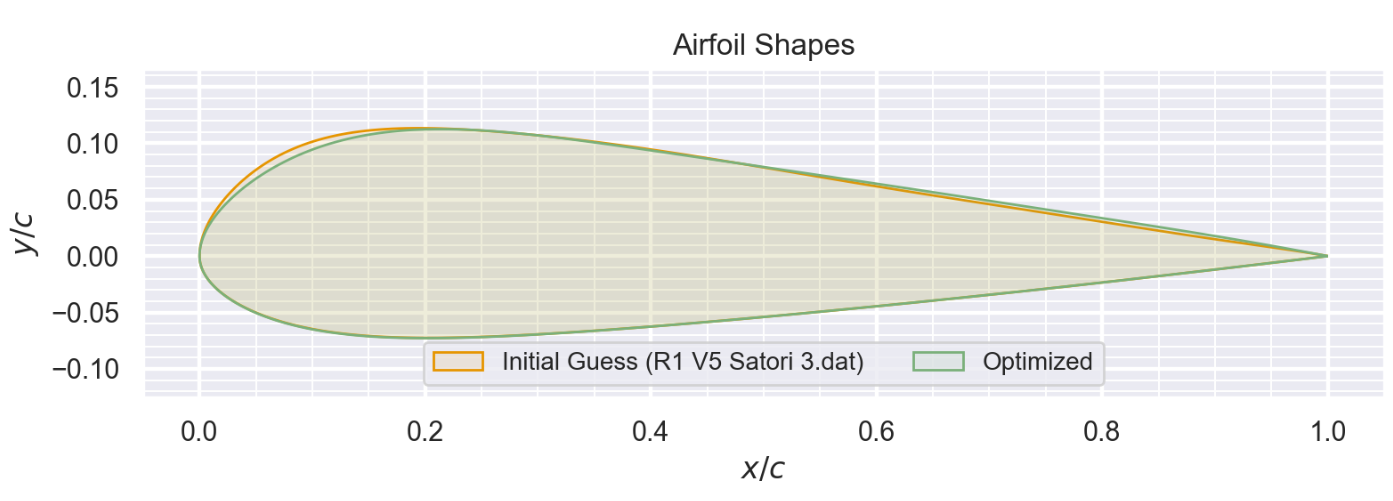
\includegraphics[width=1.\textwidth]{figures/Optimization/2D/Comparison intial guess and optimized airfoils.png}
    \caption{Comparison between the Initial Guess Airfoil and the Optimized Airfoil}
    \label{fig:Comparison between the Initial Guess Airfoil and the Optimized Airfoil}
\end{figure}

We can see on the figure \ref{fig:Comparison between the Initial Guess Airfoil and the Optimized Airfoil} that the algorithm put the apex slightly backward to increase the airfoil finesse.

As a results, simulations with Fluent were run in order to validate the airfoil before starting a new prototype : 

\begin{figure}[H]
    \centering
    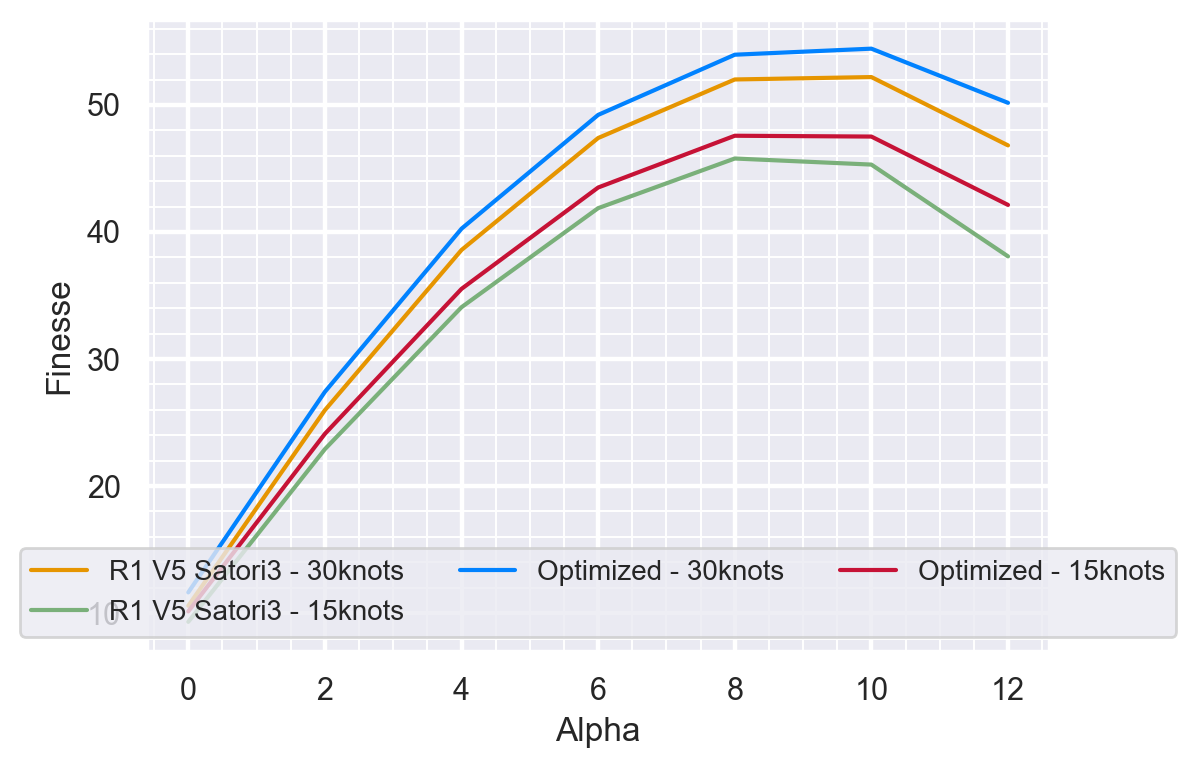
\includegraphics[width=1.\textwidth]{figures/Optimization/2D/finesse optimized and Satori3.png}
    \caption{Finesses of the R1 V5 Satori3 and the optimized airfoils (FLUENT)}
    \label{fig:Finesses of the R1 V5 Satori3 and the optimized airfoils}
\end{figure}

Figure \ref{fig:Finesses of the R1 V5 Satori3 and the optimized airfoils} suggests that the theoretically optimized airfoil should outperform the R1 V5 Satori 3. 

It's worth noting that 3D effects and actual testing may reveal unforeseen factors that could potentially impact the performance of the optimized profile. However, at this stage, there is confidence that this airfoil is an improvement over the current airfoil under evaluation.


%%%%%%%%%%%%%%%%%%%%%%%%%%%%%%%%%%%%%%%%%%%%%%%%%%%%%%%%%%%%%%%%%%%%%%%%%%%%%%%%
%%%%%%%%%%%%%%%%%%%%%%%%%%%%%%%%%%%% SECTION 3 %%%%%%%%%%%%%%%%%%%%%%%%%%%%%%%%%
%%%%%%%%%%%%%%%%%%%%%%%%%%%%%%%%%%%%%%%%%%%%%%%%%%%%%%%%%%%%%%%%%%%%%%%%%%%%%%%%

\section{3D optimization}
\label{sec:Ch2.3}

An alternative approach to enhance the performance of the R1 involves optimizing 3D parameters. I initially concentrated on optimizing the twist distribution along the span and subsequently extended the optimization to the wing's planform. 

The primary challenge associated with 3D optimization lies in the computational cost. In practice, even though VLM simulations might not appear significantly more complex at first glance, the algorithm must address 33 variables in 3D (corresponding to 33 sections along the wing's span) as opposed to the 10 variables used in 2D (related to Kulfan airfoil parameters).

This elevated level of complexity may result in outcomes that fail to converge, an excessive number of iterations, or a shortage of available computer memory space.

Additionally, the need for spatial discretization along both the wing's span and its chord required an evaluation of spatial convergence when employing the vortex lattice method before initiating the optimization of the twist distribution along the span.

\begin{figure}[H]
    \centering
    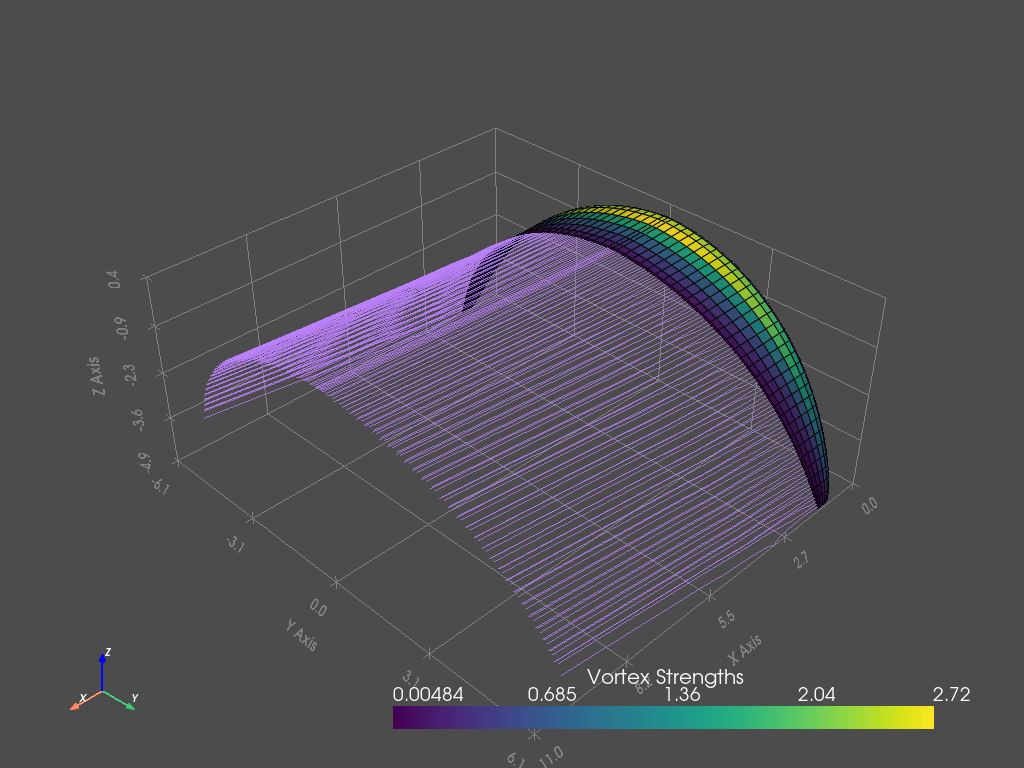
\includegraphics[width=1.\linewidth]{figures/Optimization/3D/vlm.png}
    \caption{Draw of a VLM simulation on the R1 V5 Satori 3}
    \label{fig:Draw of a VLM simulation on the R1 V5 Satori 3}
\end{figure}

%%%%%%%%%%%%%%%%%%%%%%%%%%%%%%%%%%%% SUBSECTION 1
\subsection{The spatial convergence of the VLM simulations}
\label{sub:Ch2.3.1}

Aerosandbox offers to discretize along the chord via $"chordwise\_resolution"$ and along the span via $"spanwise\_resolution"$, two parameters of the VLM function. Note that $spanwise\_resolution$ is the number of element aerosandbox considers between two sections of the wings. As the wing is defined with 33 sections, a $spanwise\_resolution$ of k means $33 * k$ elements along the span.

Therefore, VLM simulations have been run for different values of these very two parameters in order to find the values for which the simulations can be considered to have sufficiently converged to their asymptotic values.

Note that results in terms of relative error don't change with the speed or the aerodynamic coefficient we calculate.

\begin{figure}[H]
    \centering
    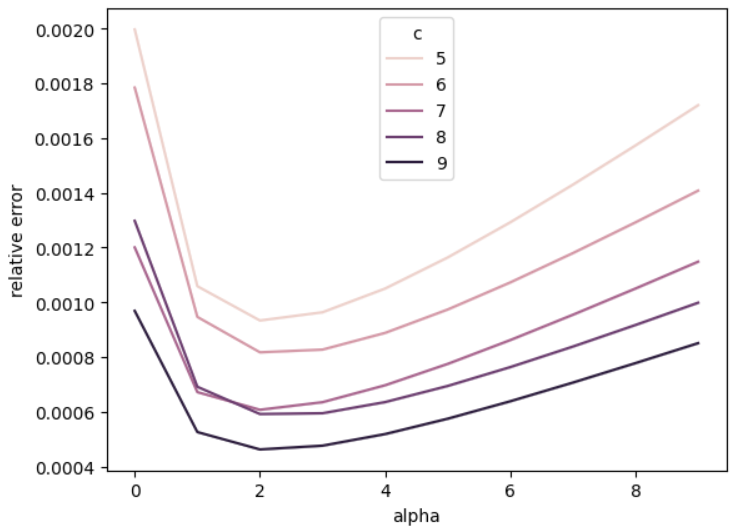
\includegraphics[width=0.8\textwidth]{figures/Optimization/3D/error_span_1_2.png}
    \caption{Relative error in lift force between a spanwise resolution of 1 and 2}
    \label{fig:Relative error in lift force between a spanwise resolution of 1 and 2}
\end{figure}

The figure \ref{fig:Relative error in lift force between a spanwise resolution of 1 and 2} shows that choosing $spanwise\_resolution = 1$ is enough to consider the simulation to have spatially converged. Note that in figures  \ref{fig:Relative error in lift force between a spanwise resolution of 1 and 2} and \ref{fig:Relative error in lift force} "c" is the $chordwise\_resolution$ parameter and "s" is the $spanwise\_resolution$ parameter.

\begin{figure}[H]
    \begin{subfigure}{0.5\textwidth}
    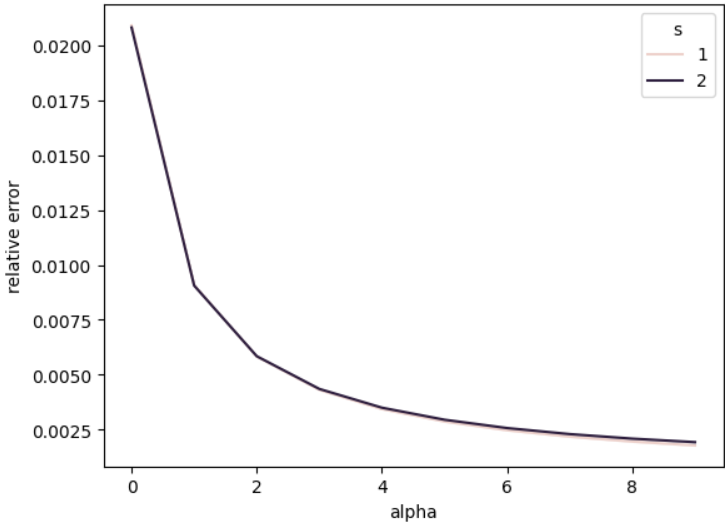
\includegraphics[width=1.\textwidth]{figures/Optimization/3D/error_chord_7_8.png}
    \caption{between chordwise resolutions of 7 and 8}
    \label{fig:between chordwise resolutions of 7 and 8}
    \end{subfigure}
    \begin{subfigure}{0.5\textwidth}
    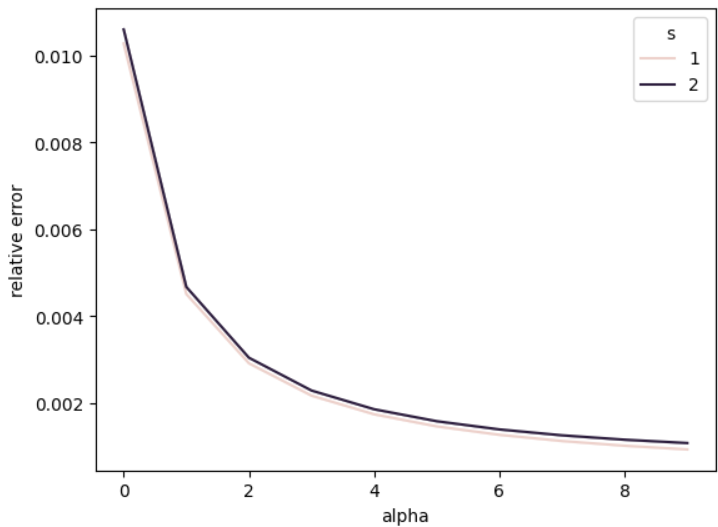
\includegraphics[width=1.\textwidth]{figures/Optimization/3D/error_chord_8_9.png}
    \caption{between chordwise resolutions of 8 and 9}
    \label{fig:between chordwise resolutions of 8 and 9}
    \end{subfigure}
    \caption{Relative error in lift force}
\label{fig:Relative error in lift force}
\end{figure}

The figure \ref{fig:Relative error in lift force} shows that we can already consider the VLM simulations to have converged for $chordwise\_resolution = 8$. This $chordwise\_resolution$ value is a good compromise between computational cost and accuracy.

\textbf{As a consequence, the following parameters have been selected for VLM simulations using Aerosandbox to achieve spatial convergence while minimizing computational costs : }
\begin{itemize}
    \item $chordwise\_resolution = 8$
    \item $spanwise\_resolution = 1$
\end{itemize}

%%%%%%%%%%%%%%%%%%%%%%%%%%%%%%%%%%%% SUBSECTION 2
\subsection{The twist optimization}
\label{sub:Ch2.3.2}

The twist optimization is intended to address the issue of reduced finesse at high angles of attack and during downwind maneuvers. Based on feedback from team riders, the existing kites do not exhibit sufficient forward flight characteristics, resulting in riders experiencing a lack of tension in the lines during their rides. Furthermore, Benoit Augier, a Ph.D. expert in fluid mechanics at the Marine Hydrodynamic Laboratory in Brest, who is currently collaborating with the French kitesurfing team for the Olympic Games, suggests that there is still room for reducing kite drag under these conditions changing the kite twist or its planform.

However, it encounters a challenge in terms of computational complexity. Unlike 2D optimizations, which typically take about 10 minutes to complete, the twist optimization algorithm requires several hours to run. If I lack the resources required to conduct simulations until we have a precise law that defines the optimal kite twist at various angles of attack, I can, however, run a simulation at a single angle of attack to obtain an initial glimpse of what such a twist profile might look like.

Therefore, I executed the optimization algorithm at a 9° angle of attack and a wind speed of 20 knots, under the following conditions :

\begin{itemize}
    \item The kite should support a load of 150 kg
    \item The $\frac{d}{d_{z}}$ of the twist cannot exceed 3°/section (a physical constraint that ensures manufacturability)
\end{itemize}

The algorithm required 62 minutes to complete.

\begin{figure}[H]
    \centering
    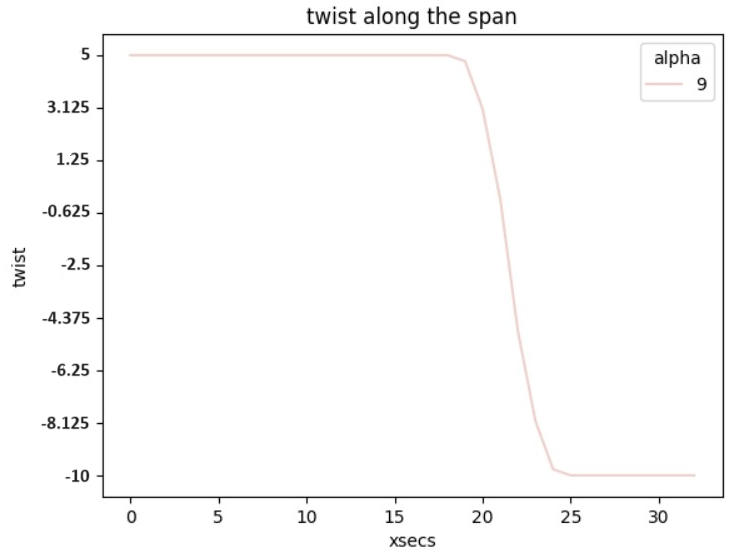
\includegraphics[width=0.7\textwidth]{figures/Optimization/3D/twist along the span.png}
    \caption{The twist distribution along the wing's span that minimizes drag at a 9° angle of attack during downwind conditions (at 20 knots)}
    \label{fig:Result of the twist law along the span the gives the minimum drag at 9° in downwind conditions (20 knots)}
\end{figure}

The figure \ref{fig:Result of the twist law along the span the gives the minimum drag at 9° in downwind conditions (20 knots)} indicates that the algorithm strives to distribute the load evenly across the kite's middle section and minimize drag resulting from tip vortices. 

Currently, these results haven't been utilized by Ozone kitesurf due to the tight deadlines the brand faces for submitting the kite sail design for the 2028 Olympic Games. However, this 3D optimization algorithm could prove beneficial for the brand if tested on their future prototypes, offering an alternative means of improving kites performances.

Furthermore, the Ozone paraglider design team is already engaged in this project, and their upcoming paraglider design may benefit from the use of this algorithm.

While planform optimization has also been implemented, it is computationally intensive and strains the capabilities of my computer. With access to more powerful computing resources, both planform and twist optimizations could be conducted simultaneously, providing the design team with a kite that fully harnesses the potential of its airfoil.

%%%%%%%%%%%%%%%%%%%%%%%%%%%%%%%%%%%% SUBSECTION 3
\subsection{The equilibrium of moments}
\label{sub:Ch2.3.3}

Another algorithm has been employed for the prediction of the kite's position within the wind window. By leveraging the knowledge of the bar position set by the athlete and applying the principles of moment equilibrium (minimizing the absolute value of the moment with an optimization algorithm) around the athlete between the kite's aerodynamic forces and the drag in the lines, we were able to compute the kite's angle of attack.

Remarkably, this algorithm achieved a prediction that had previously remained elusive for Ozone and, as far as my research indicates, for anyone in the kitesurfing community: the angle of attack of a kite and its positioning in the wind window, relying solely on the kite's aerodynamic properties without knowledge of water foil drag or athlete drag.

Consequently, the algorithm effectively validated the data in Table \ref{tab:commonly_accepted_inlet_values} and stands as a robust tool for Ozone to forecast kite flight conditions based on the athlete's speed.

\begin{figure}[H]
    \centering
    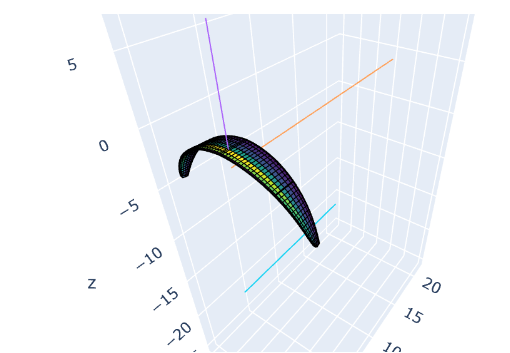
\includegraphics[width=1.\linewidth]{figures/Optimization/3D/equilibre moment.png}
    \caption{An illustration depicting the equilibrium of moments on the athlete (25 meters under the kite) (with rescaled forces)}
    \label{fig:An illustration depicting the equilibrium of moments}
\end{figure}

\begin{figure}[H]
  \begin{subfigure}{0.5\textwidth}
    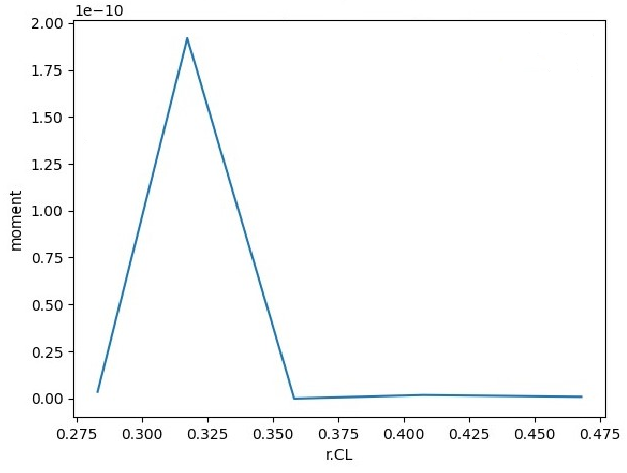
\includegraphics[width=\textwidth]{figures/Optimization/3D/moment equilibre.png}
    \caption{Moment (Nm) against Cl}
  \end{subfigure}
  \begin{subfigure}{0.5\textwidth}
    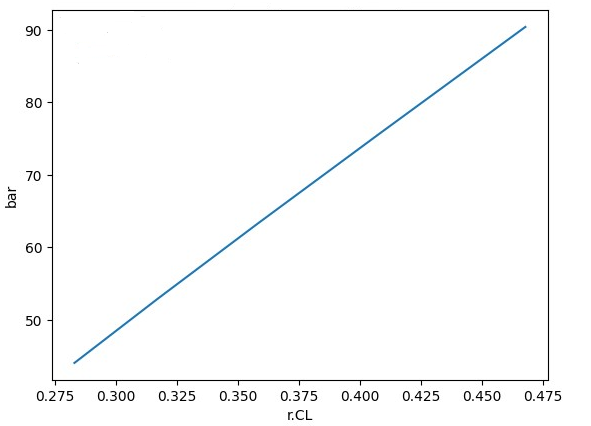
\includegraphics[width=\textwidth]{figures/Optimization/3D/moment equilibre bar.png}
    \caption{Bar position (cm) against Cl}
  \end{subfigure}
  \begin{subfigure}{0.5\textwidth}
    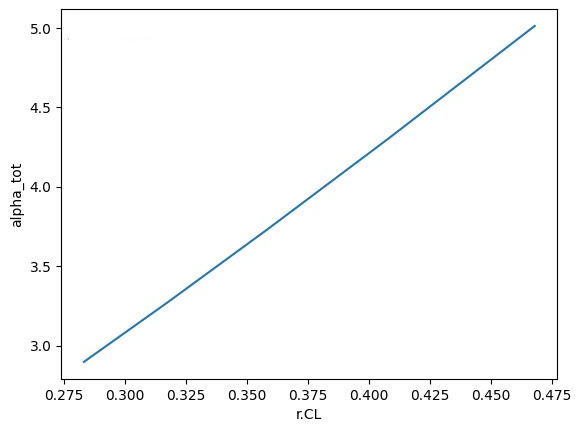
\includegraphics[width=\textwidth]{figures/Optimization/3D/moment equilibre alpha.png}
    \caption{Angle of attack (°) against Cl}
  \end{subfigure}
  \caption{Plots at 35 knots (Upwind conditions)}
  \label{Plots at 35 knots (Upwind conditions)}
\end{figure}

The information presented in Figure \ref{Plots at 35 knots (Upwind conditions)} clearly indicates that, under upwind conditions, and with an offset applied to the bar position to attain the actual kite deformation, the kite's angle of attack falls within the range of 0° to 5°, aligning with the predictions detailed in Table \ref{tab:commonly_accepted_inlet_values}.